\section{Overview of Plasma Physics}
A \emph{plasma} is a quasi-neutral gas of ions, electrons, and neutral particles, which exhibit collective behavior. A plasma can behave in similar ways to a conventional fluid -- they can flow, they can be compressible, they can be turbulent, and so on -- however the addition of charged particles facilitates many behaviors unique to a plasma. Charged particles can interact with each other not just through ballistic collisions, but at a distance through electromagnetic forces. The bulk motion of a plasma can be manipulated through electric and magnetic fields; conversely a plasma can have a substantial effect on the propagation of radio waves passing through it. 

A plasma can be analyzed in several different domains: Single particle motion; fluid approximations; and full kinematic solutions. In this work we treat the motions of electrons in the single particle domain, which is a natural choice for the sparse densities and small gyroradii of radiation belt electrons. To understand the behavior of radio waves propagating through a plasma, we treat the background as a smooth dielectric medium. 

\subsection{Single-Particle Motion}
The high energies and sparse densities of the radiation belts lend themselves very well to a single-particle approximation. Many of the basic behaviors and quantities in plasma physics can be understood through studying the motion of a single particle.

The fundamental equation of motion for a charged particle in an electromagnetic field is given by the Lorentz force:
\begin{equation}
\vec{F} = \frac{d\vec{p}}{d\emph{t}} = q(\vec{E} + \vec{v}\times\vec{B})
\label{eqn:lorentz_force}
\end{equation}
Where $q$ represents the particle's charge, $\vec{E}$ and $\vec{B}$ represent the electric and magnetic fields, and $\vec{v}$ the particle's velocity, shown here in a non-relativistic frame.

Electric fields simply apply a force in the direction of the field. However, note that a cross product is perpendicular to both terms -- therefore any forces induced by the magnetic field will be perpendicular to the particle's velocity. The magnetic field is a \emph{conservative} force, in that a stationary magnetic field cannot directly impart energy into a particle, but can alter a particle's trajectory. The particle will therefore have a net drift in the direction of the electric field, while exhibiting a helical motion around the magnetic field.

We can then split the velocity vector into two quantities -- $v_\parallel$ parallel to the magnetic field, and $v_\perp$ perpendicular to the magnetic field.

Two characteristic values arise from this motion: the radius of the particle's rotation around the magnetic field, known as the \emph{gyroradius} or the \emph{Larmor radius}:
\begin{equation}
r_l = \frac{m v_\perp}{qB}
\end{equation}

And the rotation frequency, known as the \emph{gyrofrequency} or \emph{cyclotron frequency}:
\begin{equation}
\omega_c = \frac{v_\perp}{r_l} = \frac{q B}{m} \unit{rad/sec}
\end{equation}

By integrating the particle's momentum over a single gyrorotation, we arrive at a third fundamental quantity known as the magnetic moment, or the \emph{first adiabatic invariant}:
\begin{equation}
\mu = \frac{m v_\perp^2}{2B}
\label{eqn:mu}
\end{equation}

In situations where the magnetic field varies slowly (e.g., on spatial scales much greater than the gyroradius), then $\mu$ remains a constant of motion.

A final parameter to describe a particle's motion is it's \emph{pitch angle}, the angle between the velocities perpendicular and parallel to the magnetic field:
\begin{equation}
\alpha = \mathrm{tan}^{-1}\bigg(\frac{v_\perp}{v_\parallel}\bigg)
\end{equation}








\subsection{Distributions and Dispersion Relations}
\section{Coordinate Systems}
\section{Lightning Illumination Model}


\subsection{Emission Spectrum}
While a terrestrial lightning flash consists of several repeated strokes at varying incident angles, we adopt the simplified model used by \cite{Lauben1998} and subsequent workers.

The lightning flash is modeled as a single, vertical current pulse from a height $H_E$, with a time profile given by equation \ref{eqn:td_pulse}:
\begin{equation}
\label{eqn:td_pulse}
I(t)=I_0(e^{-a t} - e^{-b t})
\end{equation}

We relate the time-domain current profile to radiated power using the far-field approximation for an arbitrary source, given by \cite{Griffiths1999}, page 457:
\begin{equation}
\label{eqn:griffiths_power}
S(t) \approx \frac{1}{\mu_0}(\mathbf{E} \times \mathbf{B}) = \frac{\mu_0}{16\pi^2c}\left[\ddot{p}(t)\right]^2 \left(\frac{\sin^2\theta}{r^2}\right)\mathbf{\hat{r}}
\end{equation}

where $p(t)$ is the dipole moment given by $p=2 H_E \int_0^t{I(t)}dt$, r is the distance from the flash in meters, and $\theta$ is the angle to the flash. Taking the second derivative of the dipole moment (the first derivative of the current profile) gives us the far-field time-domain power equation:

\begin{equation}
\label{eqn:farfield_power_td}
S(t) = \frac{1}{Z_0}\left(\frac{\mu_0 H_E I_0}{2 \pi}\right)^2\left(\frac{\sin^2\theta}{r^2}\right) \left(a e^{-a t} - b e^{-b t}\right)^2  \mathbf{\hat{r}}
\end{equation}

where we have used the relation $Z_0 = \mu_0 c$. Equation \ref{eqn:farfield_power_td} has units of energy flux density, Watts per square meter ($J/m^2/$sec).

To determine the frequency spectrum of the radiated power, we take the Fourier transform of equation \ref{eqn:farfield_power_td}:

\begin{equation}
\label{eqn:farfield_power_fd}
S(\omega) = \frac{1}{Z_0}\left(\frac{\mu_0 H_E I_0}{2 \pi}\right)^2\left(\frac{\sin^2\theta}{r^2}\right) \frac{\omega^2(a-b)^2}{(\omega^2 + a^2)(\omega^2 + b^2)}  \mathbf{\hat{r}}
\end{equation}

which has units of energy flux per frequency -- J/m$^2$/Hz.

Throughout this work we assume a flash height $H_E$=5 km, and model parameters $a=5\E{3}$ and $b=1\E{5}$, resulting in a spectrum peaked at approximately 4kHz; any lightning flash can be parameterized solely by its peak current $I_0$ and its location on the surface of the Earth. Figure \ref{fig:lightning_spectrum} shows the current profile and associated spectrum.

\begin{figure}[ht]
\begin{center}
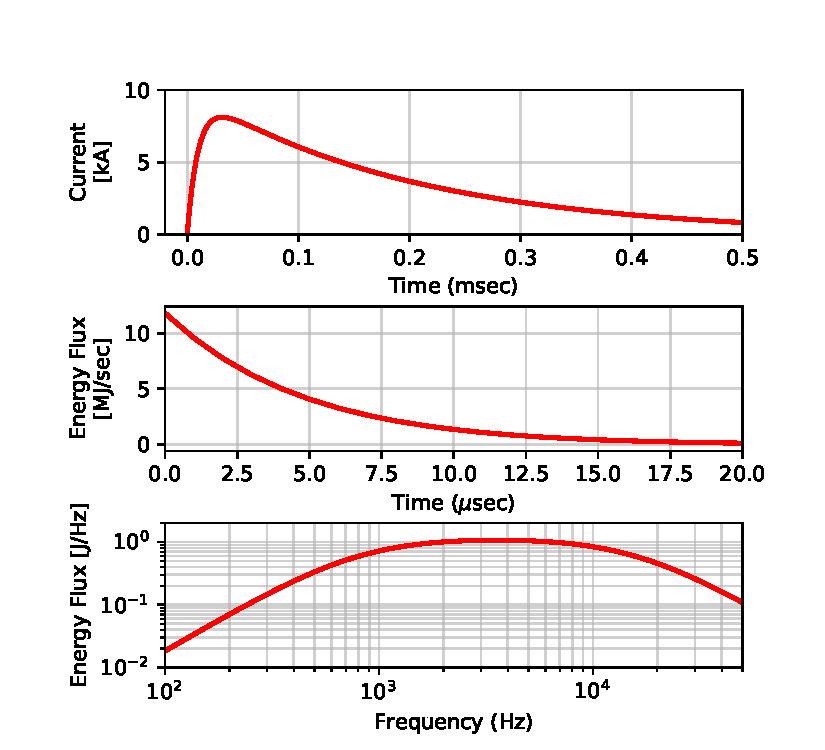
\includegraphics{figures/Lightning_spectra.pdf}

\caption{default}
\label{fig:lightning_spectrum}
\end{center}
\end{figure}

\subsection{Trans-Ionosphere Attenuation}

\section{Ray Tracing and Landau Damping}
\section{Wave-Particle Interactions}
\section{Environment Models}
\subsection{Magnetic Field}
\subsection{Ionosphere}
\subsection{Plasmasphere}
